\section{DER conceitual e modelo lógico}
\begin{figure}[!ht]
\centering
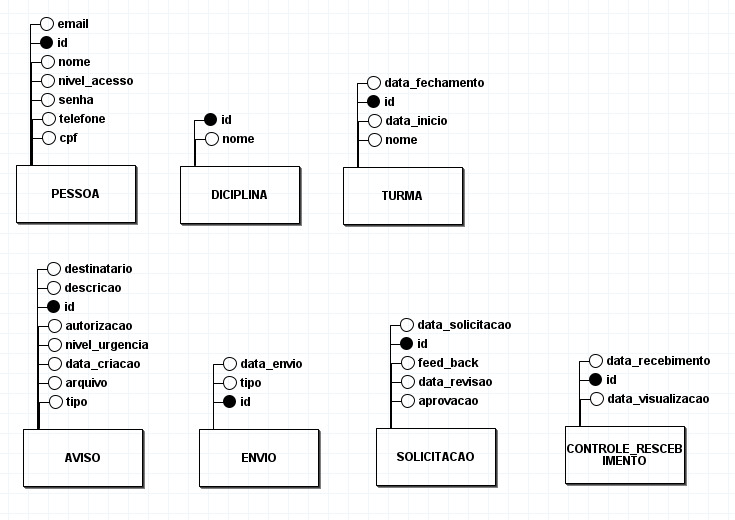
\includegraphics[width=\linewidth,height=0.62\textheight,keepaspectratio]{../../src/uml/diagrama/der.jpeg}
\caption{DER consolidado do Sistema de Comunicação Escolar.}
\end{figure}

\begin{figure}[!ht]
\centering
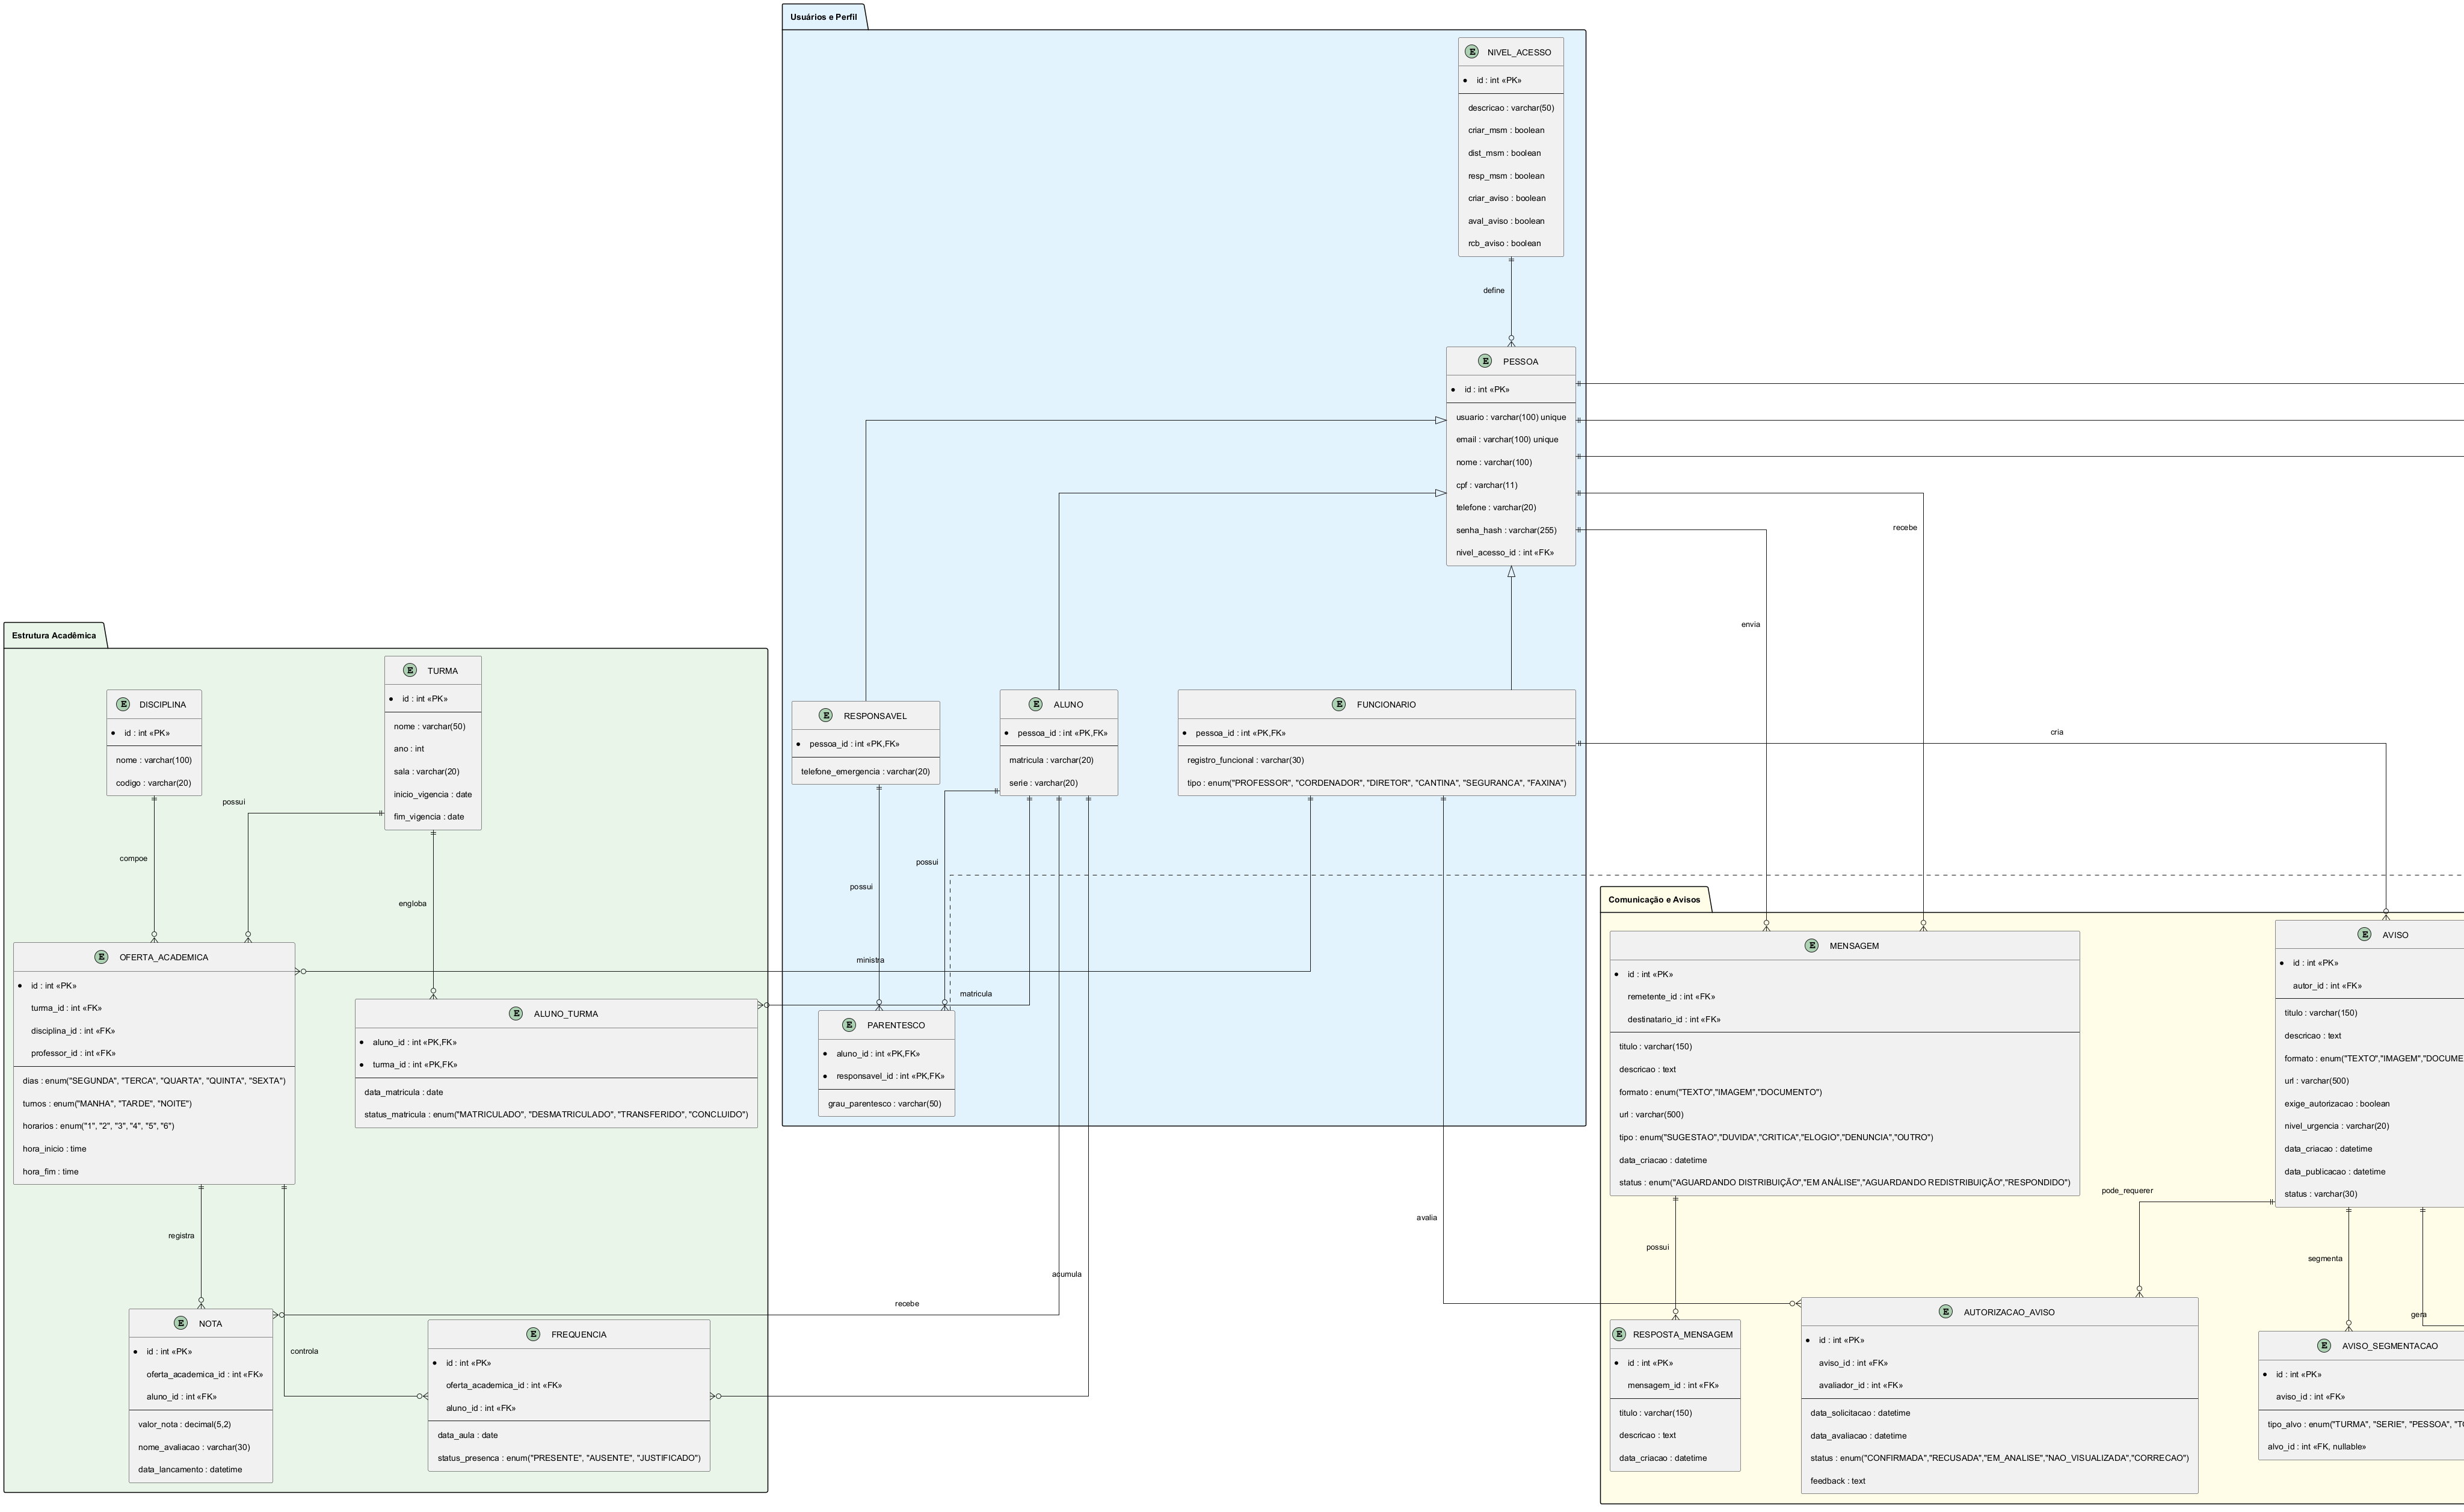
\includegraphics[width=\linewidth,height=0.62\textheight,keepaspectratio]{../../src/uml/logico/mr.png}
\caption{Modelo Relacional derivado do MER conceitual.}
\end{figure}

\begin{keyidea}[Chaves das entidades associativas]
ALUNO\_TURMA usa aluno\_id e turma\_id; ENVIO\_DESTINATARIO usa envio\_id e pessoa\_id;
CONTROLE\_RECEBIMENTO mantém referência ao par envio-destinatário. Tais entidades associativas
representam corretamente os relacionamentos muitos para muitos.
\end{keyidea}
